\section{Contrail Detection}
\label{sec:intro}

\subsection{Introduction}

Contrail detection is an essential component towards understanding the impact and mitigation of contrails. Being able to detect contrails with high accuracy is a necessary capability in order to evaluate and compare contrail predictive models, to track contrails through their lifespan and measure the amount of heat that they trap, and ultimately to verify the effectiveness of flight path diversion efforts.

Remote sensing satellites, equipped with state-of-the-art sensors, such as the Advanced Baseline Imager (ABI) on the Geostationary Operational Environmental Satellites (GOES) \cite{goes} have allowed for reliable and consistent environmental observations. Compared to Polar-orbiting Operational Environmental Satellites (POES) such as the Suomi or Sentinel satellites, GOES maintains constant observation over a fixed area with relatively higher temporal resolution but at the cost of lower spatial resolution. With 2 kilometer spatial resolution in the infrared bands, GOES imagery in not sufficient to capture the initial formation of young contrails, but is able to capture the more mature stages of contrails if they continue to spread out. GOES's coarser resolution narrows our focus on the contrails with the largest climate impact since persistent contrails that have expanded sufficiently to be observable at 2 kilometer resolution are associated with more significant warming effects \cite{warm, persist}. Additionally, the proposed contrail predictive model will be at 3 kilometer resolution, thus reducing the utility of higher resolution contrail detection. 

\subsection{Related Work}

In the last 25 years, contrails have primarily been detected in POES imagery using image processing techniques such as the Mannstein et al. algorithm \cite{mannstein} that applies a series of hand engineered convolution and thresholding operations to infrared imagery. More recently, a method for tracking the life cycle of contrails that uses the aforementioned Mannstein et al. algorithm on POES imagery for early stage detection and then uses a tracking algorithm on GOES imagery for later stage contrail evolution \cite{track}. POES satellites are often constrained by a single pass per day over a given area of interest, limiting the ability to support contrail avoidance.

With the introduction of large human-labeled contrail datasets \cite{opencontrails, landsat}, more recent studies have applied deep learning based contrail detection models \cite{opencontrails, covid} with GOES imagery. While deep learning approaches have the potential to better support contrail avoidance predictions, there has not been a direct performance analysis between the Mannstein et al. method and the deep learning models. Quantifying the effectiveness of contrail detection methods is crucial for accurate assessment of the cost and benefits of contrail predictive models. False positives of a high probability area for contrail formation would increase costs of fuel consumption for flights to take unnecessary avoidance measures. False negatives, where a flight creates preventable contrail formations, would decrease the utility of implementing contrail predictive models. 


\begin{figure}
\centering

\begin{subfigure}[t]{.49\linewidth}
  \centering
    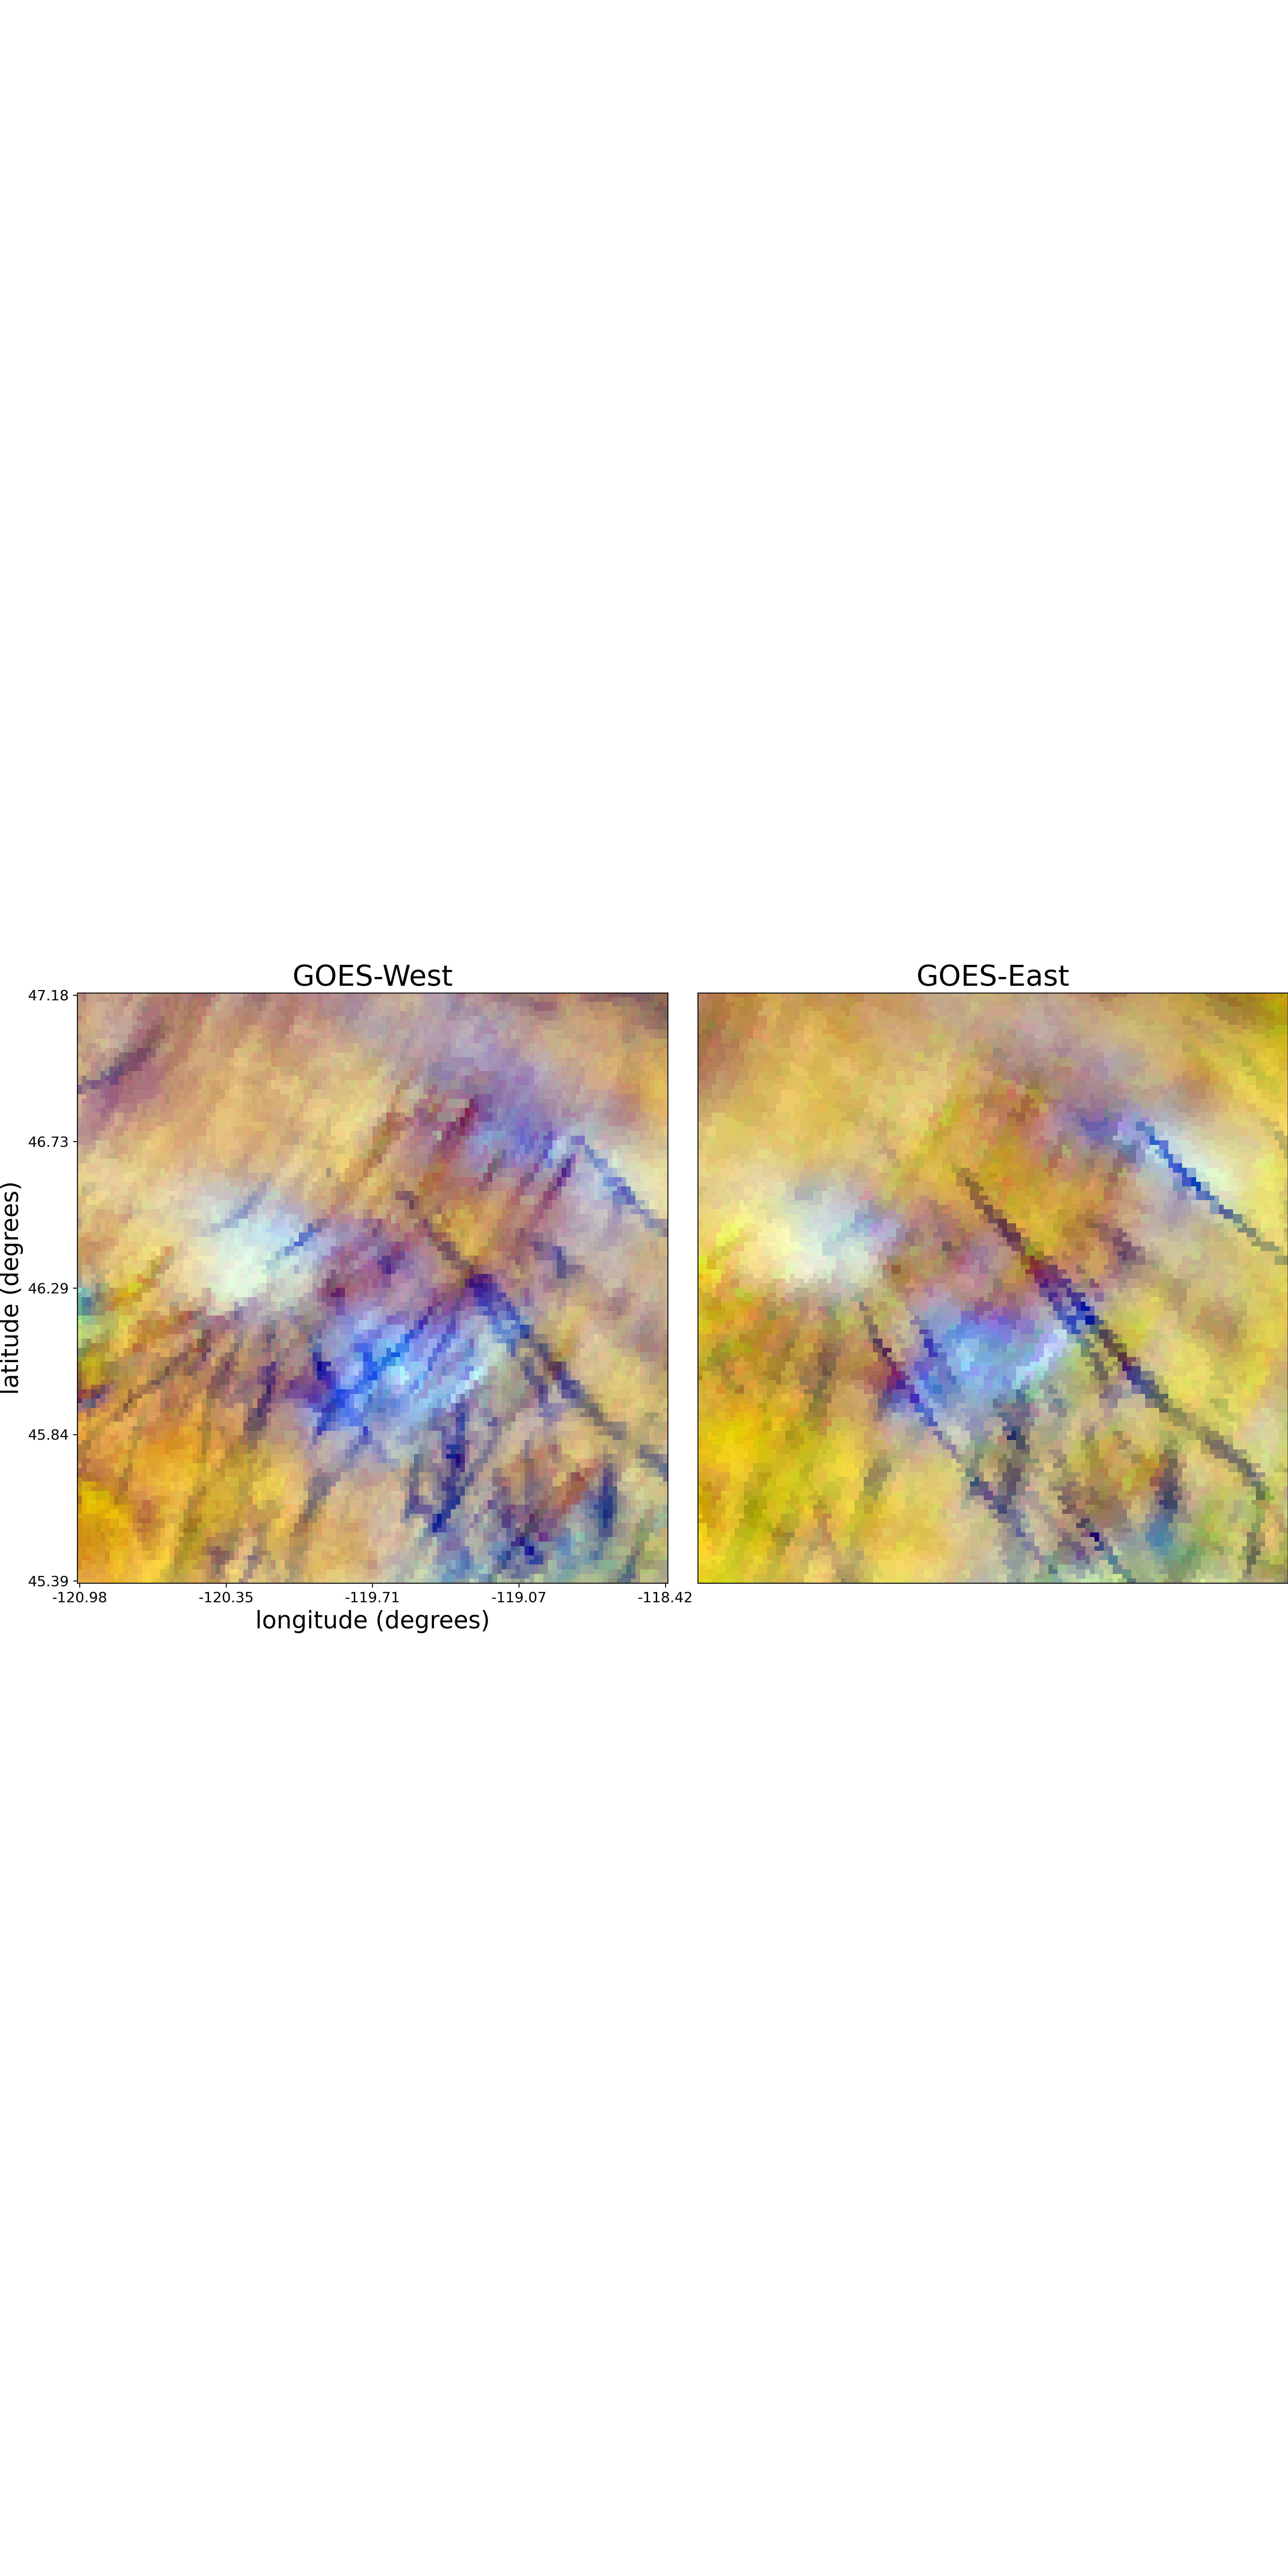
\includegraphics[width=\linewidth]{figures/west_best.png}
    \caption{GOES imagery from 2025/03/11 15:50 UTC.}
  \label{best_west}
\end{subfigure}
\hspace{.01cm}
\begin{subfigure}[t]{.49\linewidth}
  \centering
    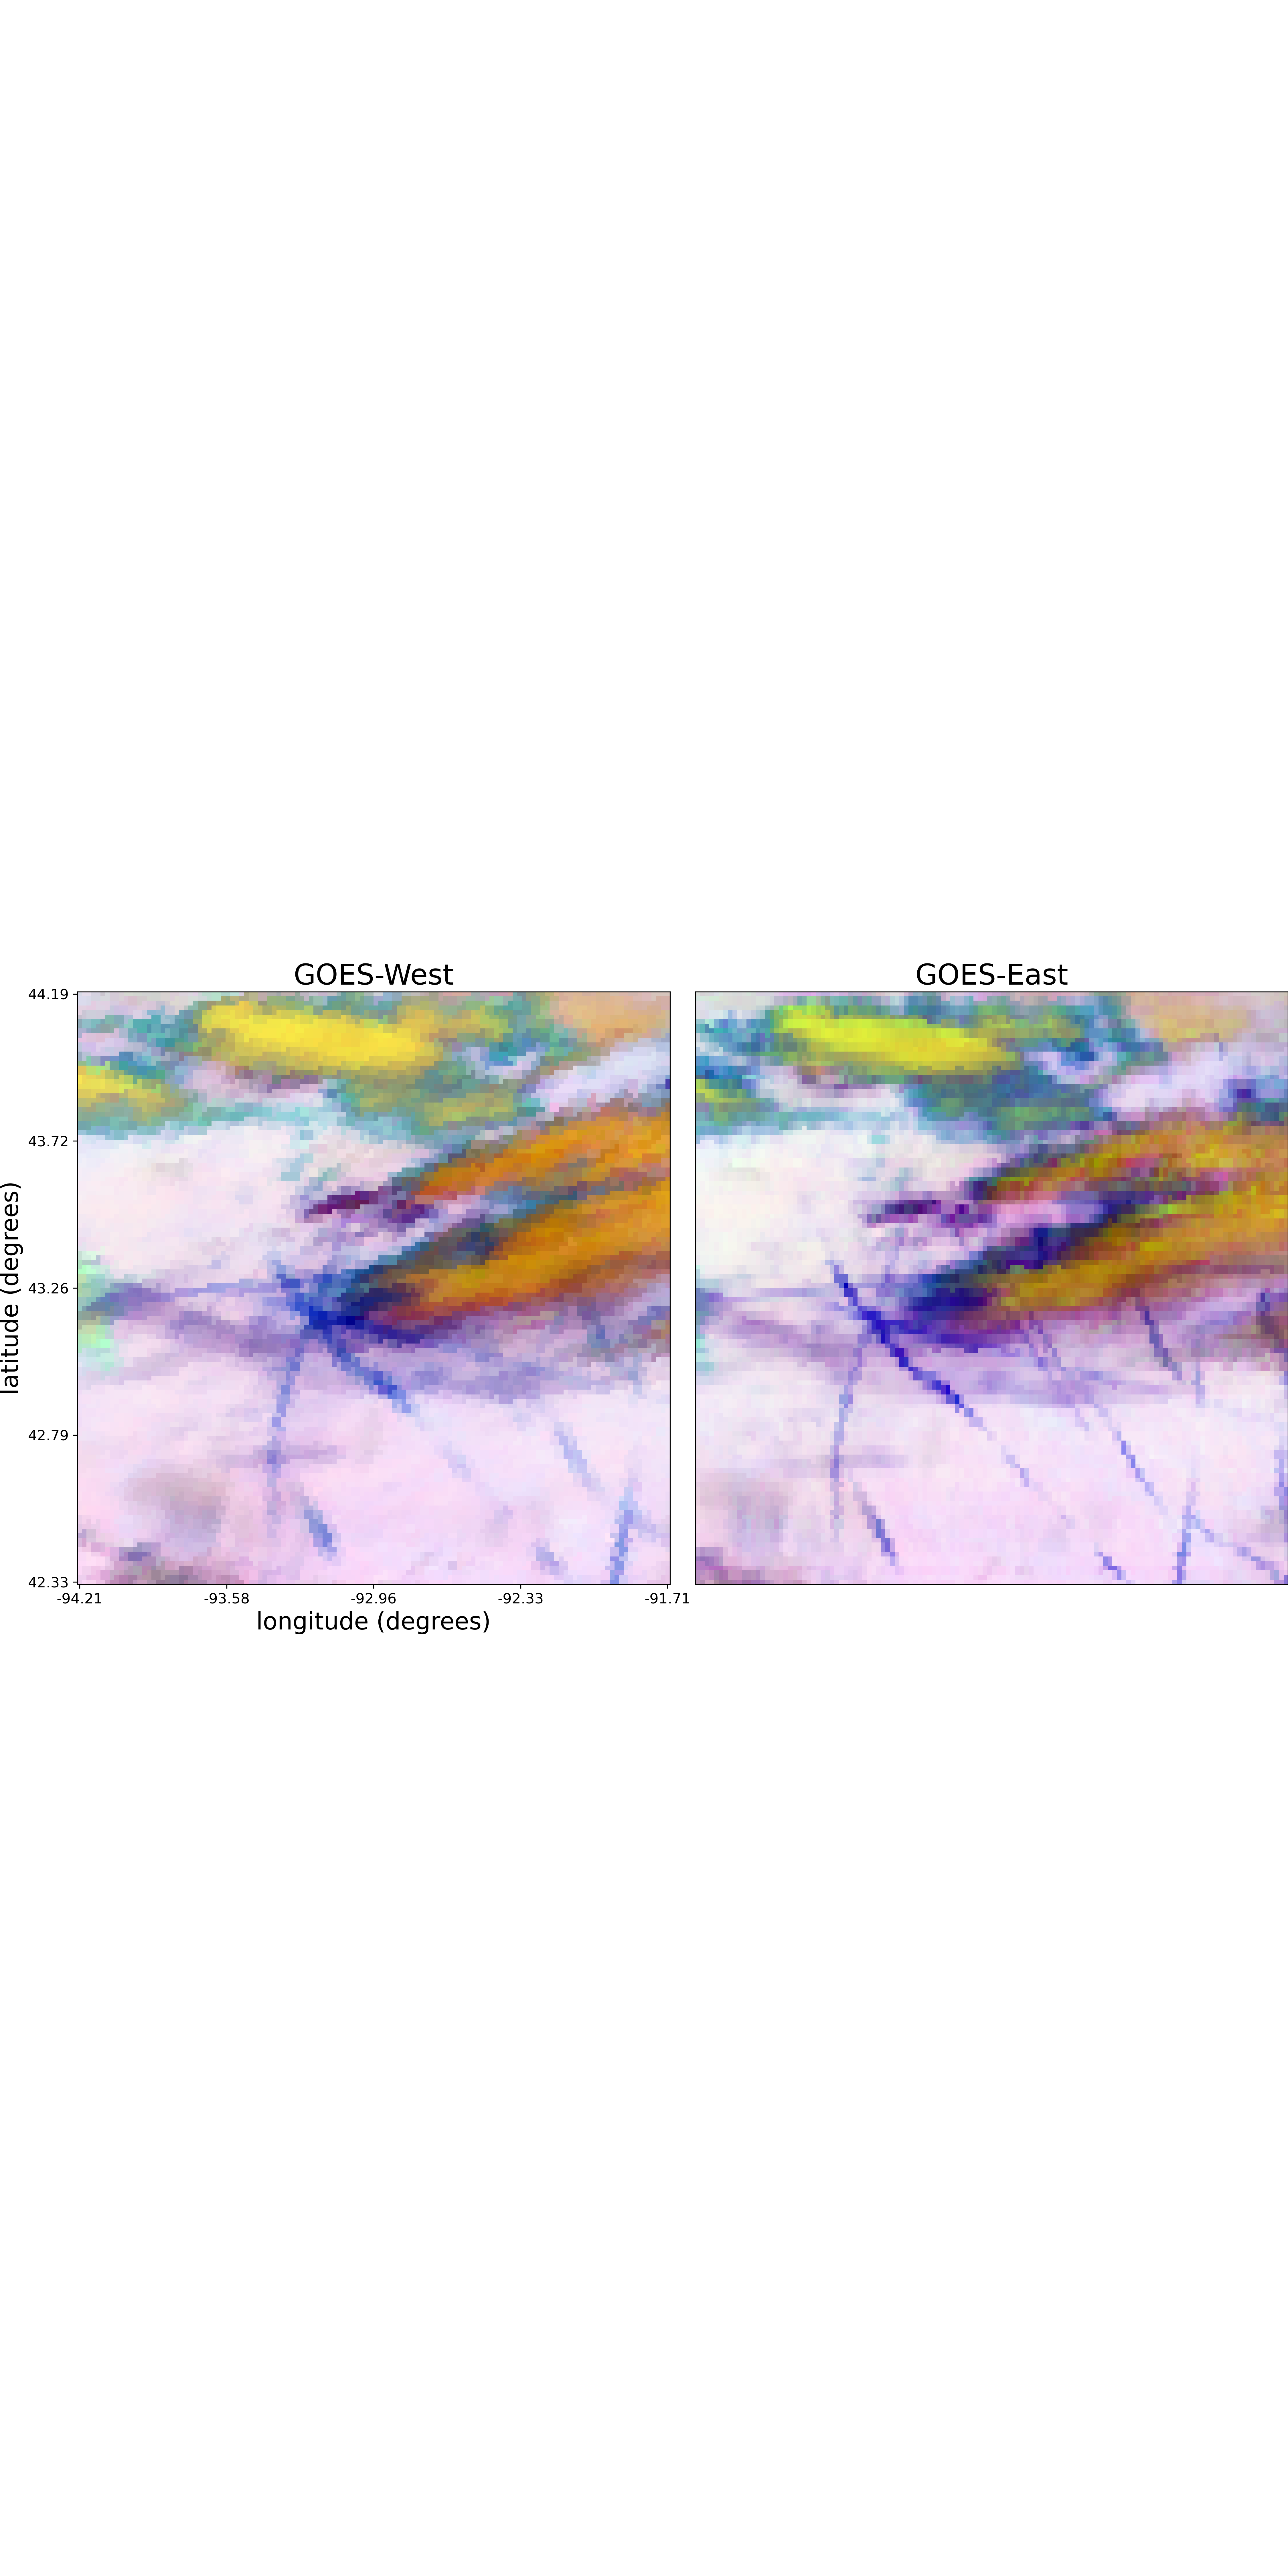
\includegraphics[width=\textwidth]{figures/east_best.png}
    \caption{GOES imagery from 2025/02/28 13:30 UTC.}
  \label{best_east}
\end{subfigure}

\begin{subfigure}[t]{.49\linewidth}
  \centering
    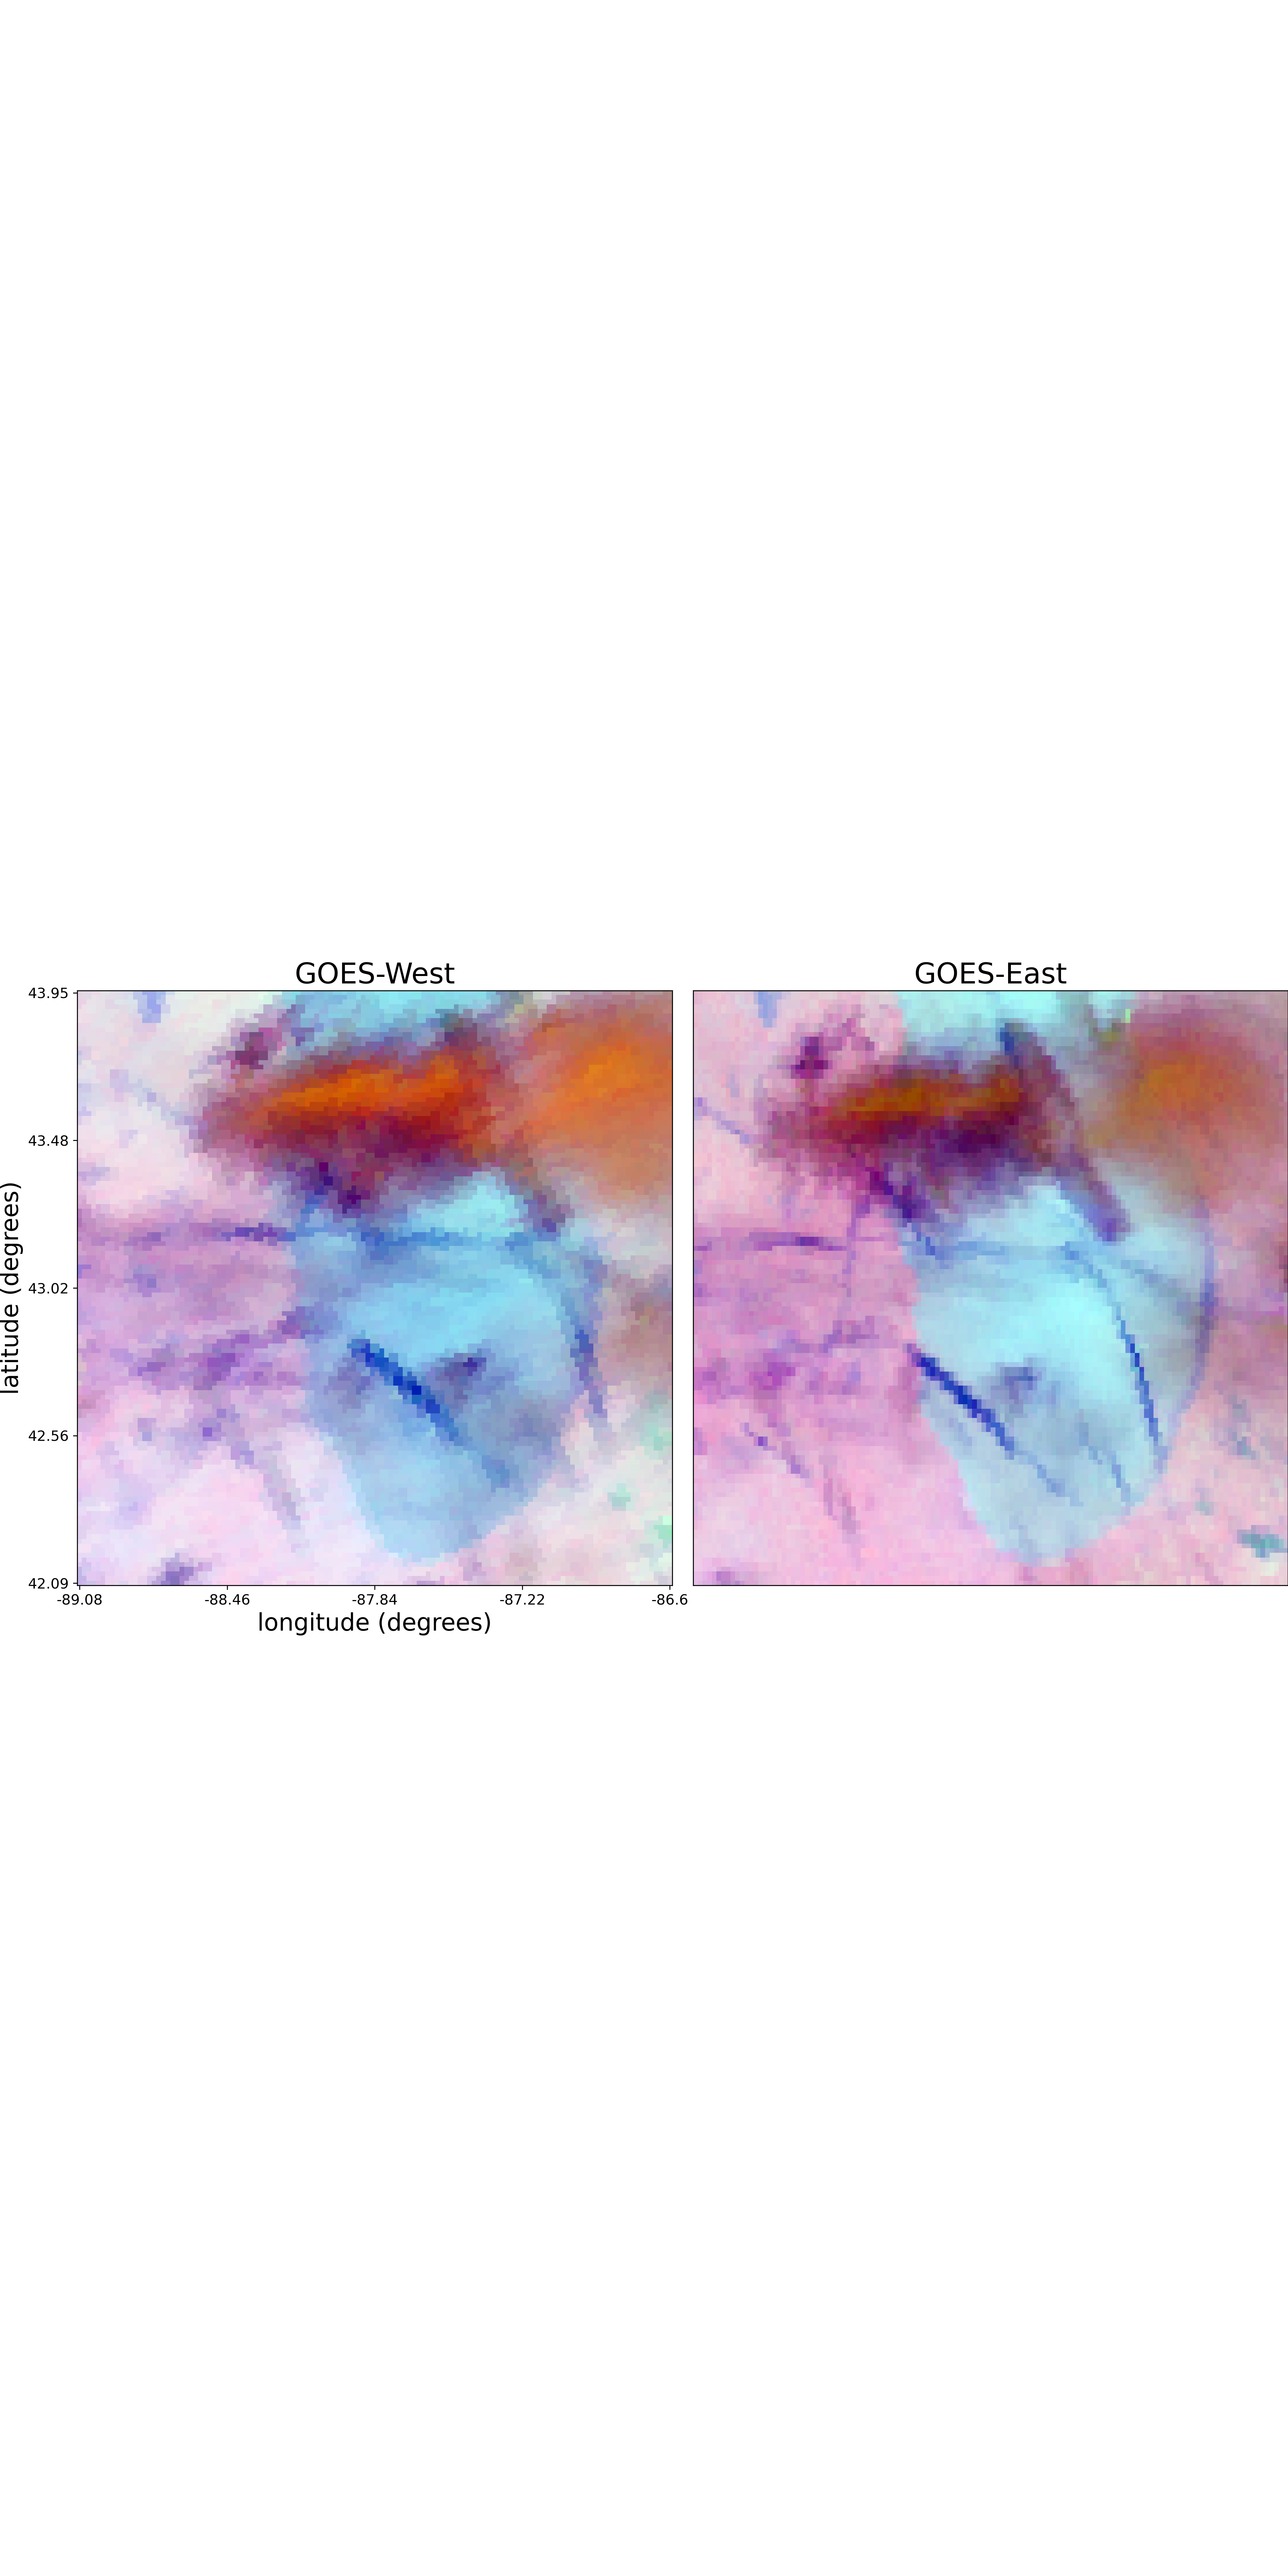
\includegraphics[width=\textwidth]{figures/superior_parallax.png}
    \caption{GOES imagery from 2025/02/28 05:40 UTC with contrails over Lake Michigan to visualize the parallax difference between GOES-West and GOES-East.}
  \label{parallax1}
\end{subfigure}
\hspace{.01cm}
\begin{subfigure}[t]{.49\linewidth}
  \centering
    \includegraphics[width=\textwidth]{figures/superior_parallax_2.png}
    \caption{Same as figure \ref{parallax1} but with contrail labels from GOES-West (black) and GOES-East (white) with the parallax distance in red corresponding to a difference of 16 pixels or 32 km.}
  \label{parallax2}
\end{subfigure}

\caption{Side-by-side comparisons of ash composites for GOES-West and GOES-East imagery using bands 11, 13, 14 and 15 (8.4\(\mu\)m, 10.3\(\mu\)m, 11.2\(\mu\)m and 12.3\(\mu\)m) to show cirrus as dark blue.}
\label{goes_img}
\end{figure}

\subsection{Proposed Work}

\subsubsection{GOES-East Deep Learning Detection Model}
While the OpenContrail project has made their GOES-East dataset publicly available, they have not shared the models they present in their paper \cite{opencontrails}. The first step towards supporting contrail prediction models will be to train a deep learning contrail detection model using state-of-the-art computer vision methods on the OpenContrails dataset. The input to the model will be GOES-East imagery for a given time window and the output will be a geospatial vector file with the geometry of detected contrails within that time window.

\subsubsection{Analysis of Mannstein et al. Algorithm}
Given the importance of accurate contrail detection models, we propose to perform a thorough analysis on how the Mannstein et al. algorithm performs on the human-labeled OpenContrail dataset. Since deep learning algorithms are only as accurate as their datasets, assessment on the quality of training data will give insight on the reliability of the resulting model. The algorithm was developed for the difference between AVHRR bands with center wavelengths around 12\(\mu\)m and 10.8\(\mu\)m at 1km resolution \cite{mannstein}. We would need to perform minimal changes to get the algorithm compatible with bands 15 (12.3\(\mu\)m) and 13 (10.3\(\mu\)m) available on the GOES-ABI.

\subsubsection{GOES-West Derived Dataset and Model}
The OpenContrail model only utilizes GOES-East imagery, but GOES-West can provide higher quality observations of the West coast (figure \ref{best_west}) with a corresponding relationship for GOES-East on the East coast (figure \ref{best_east}). Preliminary figures, \ref{best_west} and \ref{best_east}, demonstrate how contrails can be observable in one satellite but not the other. The OpenContrail dataset only provides annotations associated with GOES-East, missing contrails only visible by GOES-West. Due to the parallax effect (figure \ref{parallax1}-\ref{parallax2}) between GOES-East and West for high altitude clouds such as contrails, it is not possible to immediately match up the contrail labels to the GOES-West imagery. We will need to solve for the shift in observed location in order to build the GOES-West dataset. From that newly introduced dataset, we will then train a model that will detect contrails in GOES-West imagery. This will allow to compare the GOES-West model to the GOES-East model and provide a tool for analysis on how the parallax shift provide information on contrail altitude.

\subsubsection{Contrail Altitude Approximation from Satellite Observation}
Since predictive models are determining the altitude of a high probability area for contrail formation, it's important to have accurate altitude information to correlate with a contrail detection. In high flight traffic areas, it can be difficult to match the contrail to its correct flight data to obtain corresponding altitude information. Furthermore, even when accurately determined, it is computationally intensive to find the data that is often on a delayed release. It'd be optimal to be able to determine the altitude directly from the satellite imagery itself. We show in figure \ref{parallax2} that if we are able to match the GOES-West contrail detection to the corresponding GOES-East detection, we will be able to determine the parallax distance which is a function of the contrails altitude.

\subsubsection{Study Highest Impact Contrails}
While the primary focus of this study is to predict and mitigate persistent contrails observable by GOES's 2km resolution, we are also interested in understanding the atmospheric conditions required for persistent contrails to continue evolving into lasting fields of cirrus clouds. When contrails form cirrus fields, the radiative impact is larger than the general persistent contrail. We propose to use an existing cloud regime classification model to match contrail detections to down-the-line areas of cirrus clouds. 

